\subsubsection*{16.a}
On affecte le role SUBSCRIBE\_MANAGER a l'utilisateur admin

\lstinputlisting[style=sqlstyle]{SQL/Partie4/grantrole.sql}

\begin{center}
    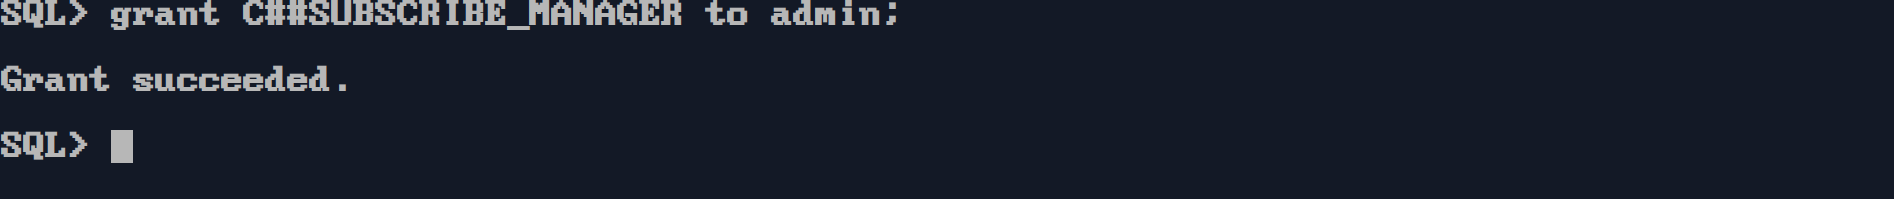
\includegraphics[width=\textwidth]{ScreenShot/Partie4/grantrole.png}
\end{center}

\subsubsection*{16.b}
les role des utilisteur sont stockes dans les table USER\_ROLE\_PRIVS et DBA\_ROLE\_PRIVS , probleme et que
admin ne peut pas creer de session donc on ne peut pas se connecter en tant que admin et afficher USER\_ROLE\_PRIVS
, et dbaiot n'est pas DBA pour acceder a DBA\_ROLE\_PRIVS , donc on se connect en tant que sysdba et afficher  
DBA\_ROLE\_PRIVS  avec WHERE GRANTEE = 'ADMIN' pour afficher just celle d'admin

\lstinputlisting[style=sqlstyle]{SQL/Partie4/verifyrole.sql}

\begin{center}
    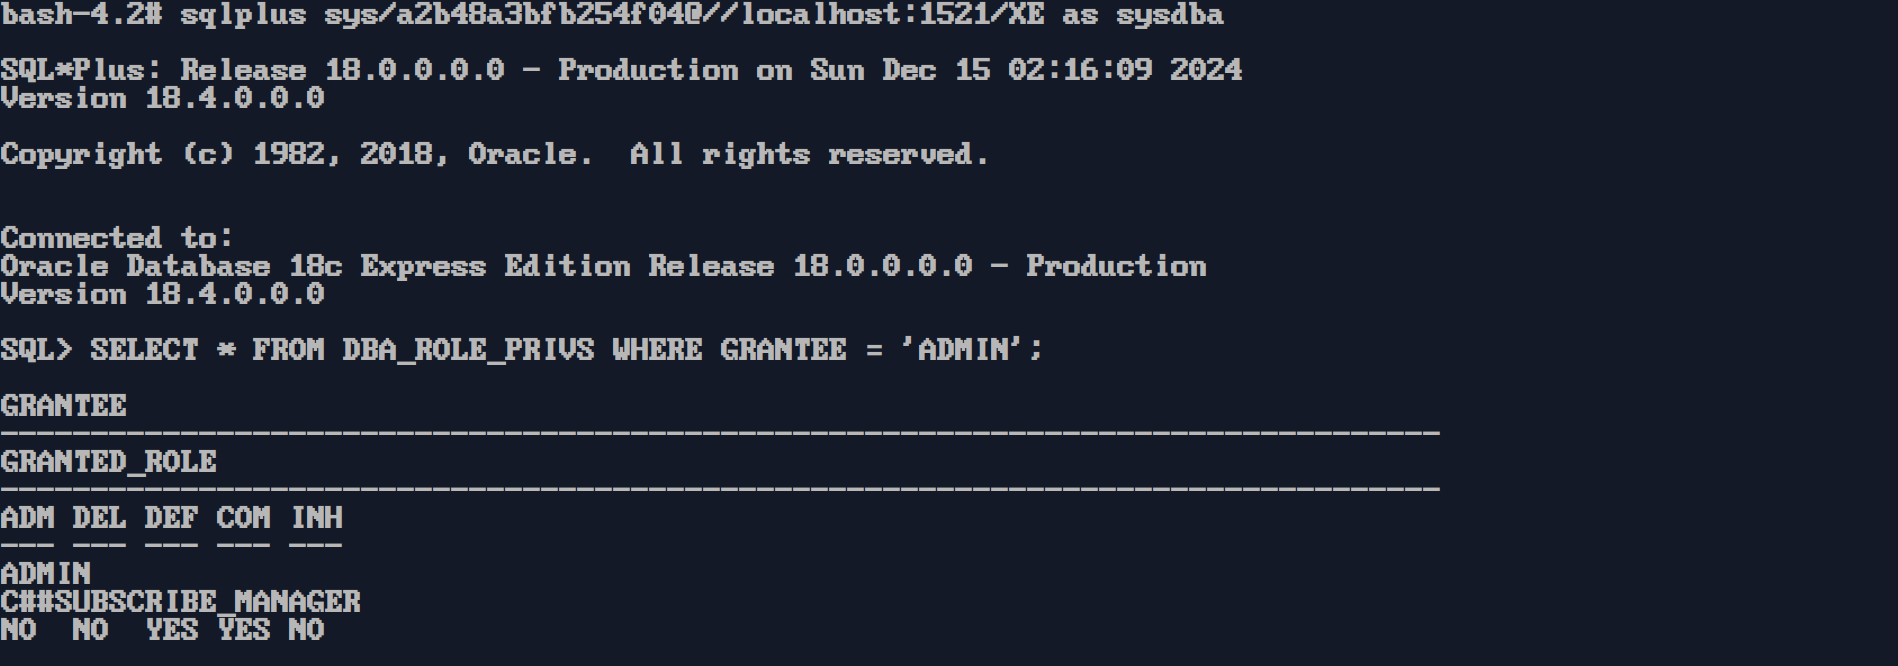
\includegraphics[width=\textwidth]{ScreenShot/Partie4/verifyrole.png}
\end{center}

\begin{prettyBox}{}{myblue}
Depuis l'output on remarque que admin a le role C\#\#SUBSCRIBE\_MANAGER
\end{prettyBox}


